% \textbf{\underline{OZ 5 - Magnetische inductie en de wet van Faraday - Oefening 2:}}
% \vspace{0.5cm}

% Een rechthoekige spoel heeft een weerstand $ R $ en bestaat uit $ N $ windingen van lengte $ l $ en breedte $ w $, zoals aangegeven op Figuur 5.2. De spoel wordt een uniform magnetisch veld $ \vec{B} $ ingeschoven met een constante snelheid $ \vec{v} $. Wat is de grootte en richting van de totale magnetische kracht op de spoel wanneer de spoel

% \begin{enumerate}[(a)]
%     \item het magnetische veld binnenkomt?
%     \item volledig in het magneetveld beweegt?
%     \item het magnetische veld verlaat?
% \end{enumerate}

% \begin{figure}[H]
%     \centering
%     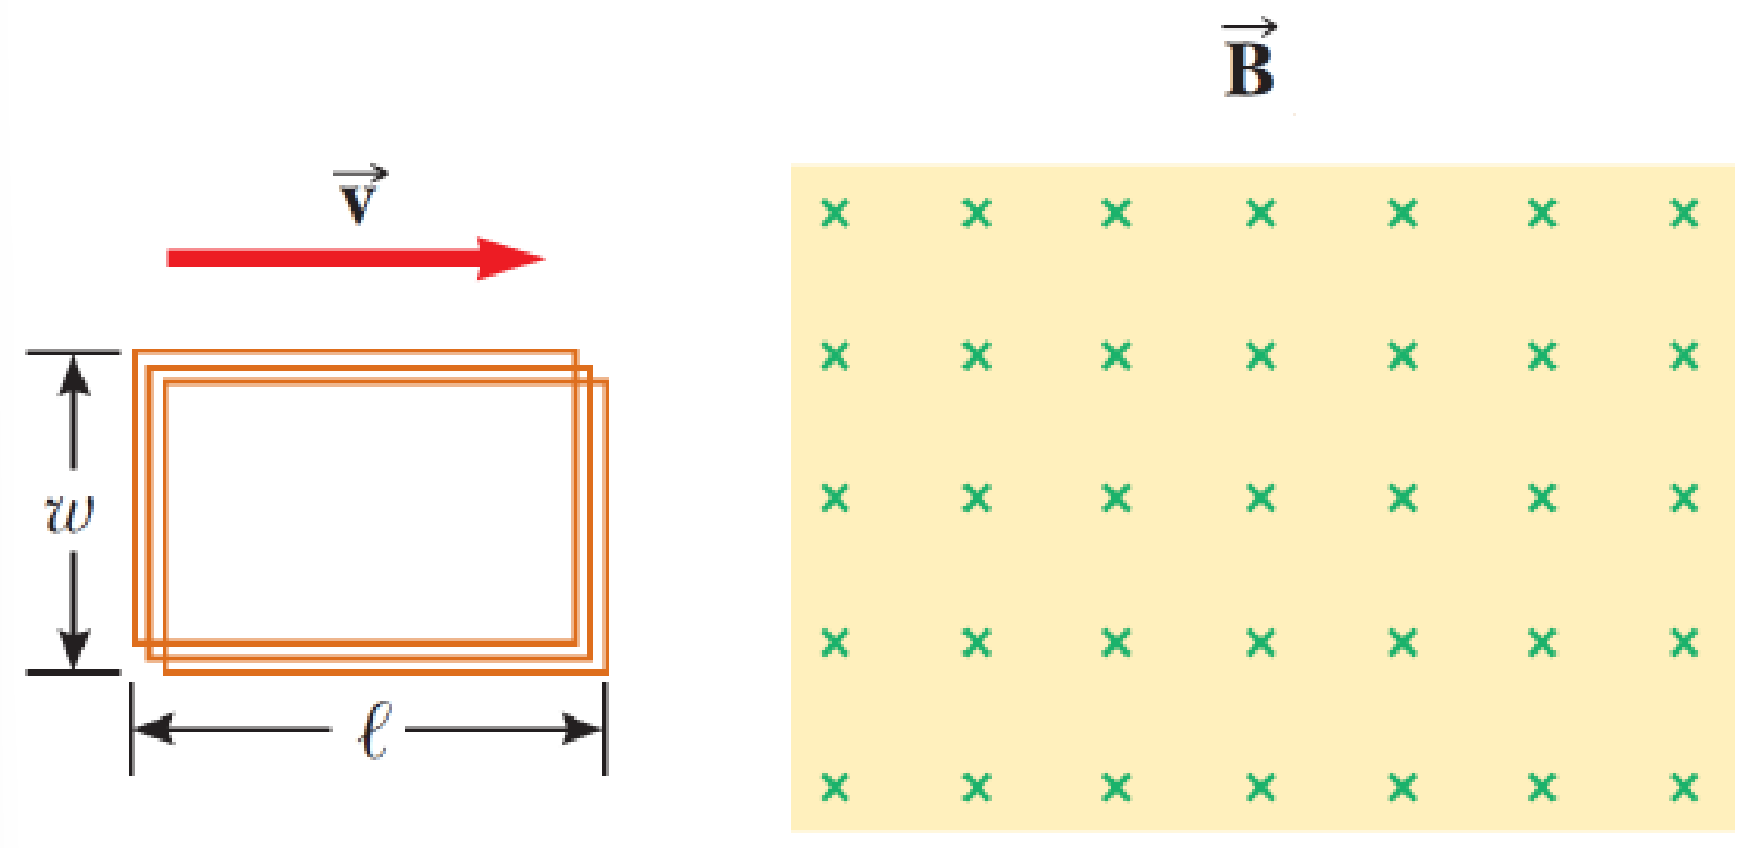
\includegraphics[width=7cm]{oz05/resources/oef-2-opgave.png}
    
%     \textbf{Figuur 5.2}
% \end{figure}

% \begin{description}[labelwidth=1.5cm, leftmargin=!]
%     \item[Geg. :]   $ R $; $ N $; $ l $; $ w $; $ \vec{B} $; $ \vec{v} $;
% \end{description}

% \begin{enumerate}[(a)]
%     \item
%         \begin{description}[labelwidth=1.5cm, leftmargin=!]
%             \item[Gevr. :]  $ \vec{F} $ bij binnenkomst;
%             \item[Opl. :]   Berekening voor 1 enkele lus:
                            
%                                 \hspace{1cm} 
%                                 $ \Phi_{B,0} = 0 $ T
                    
%                                 \hspace{1cm} 
%                                 $ \Phi_{B,e} = \int{\vec{B} \cdot d\vec{A}} = B\cdot A \cdot \cos{0^{\circ}} = B \cdot A $
                                
%                                 \hspace{1cm} 
%                                 $ dt = \dfrac{l}{v} $
                                
%                                 \hspace{1cm} 
%                                 $ \dfrac{d\Phi_B}{dt} = \dfrac{B \cdot A}{\dfrac{l}{v}} = B \cdot w \cdot v $
                            
%                             $ \varepsilon = -N \dfrac{d\Phi_B}{dt} = -N \cdot B \cdot w \cdot v $
                            
%                             $ I = \dfrac{\varepsilon}{R} = \dfrac{-N \cdot B \cdot w \cdot v}{R} $
                            
%                             $ E = P dt = I^2 R dt = \dfrac{N^2 \cdot B^2 \cdot w^2 \cdot v^2}{R} \cdot \dfrac{l}{v} 
%                             = \dfrac{N^2 \cdot B^2 \cdot w^2 \cdot v \cdot l}{R} $
                            
%                             $ F = \dfrac{W}{l} = \dfrac{\dfrac{N^2 \cdot B^2 \cdot w^2 \cdot v \cdot l}{R}}{l} = \dfrac{N^2 \cdot B^2 \cdot w^2 \cdot v}{R} $
                            
%                             $ \vec{F} = F \left( -\hat{\imath} \right) = \dfrac{N^2 \cdot B^2 \cdot w^2 \cdot v}{R} \left( -\hat{\imath} \right) $
%         \end{description}
%     \item
%         \begin{description}[labelwidth=1.5cm, leftmargin=!]
%             \item[Gevr. :]  $ \vec{F} $ volledig in het veld;
%             \item[Opl. :]   Berekening voor 1 enkele lus:
                            
%                                 \hspace{1cm} 
%                                 $ \Phi_{B,0} = \int{\vec{B} \cdot d\vec{A}} = B\cdot A \cdot \cos{0^{\circ}} = B \cdot A $
                    
%                                 \hspace{1cm} 
%                                 $ \Phi_{B,e} = \int{\vec{B} \cdot d\vec{A}} = B\cdot A \cdot \cos{0^{\circ}} = B \cdot A $
                                
%                                 \hspace{1cm} 
%                                 $ dt = \dfrac{l}{v} $
                                
%                                 \hspace{1cm} 
%                                 $ \dfrac{d\Phi_B}{dt} = \dfrac{B \cdot A - B \cdot A}{\dfrac{l}{v}} = 0 $
                            
%                             $ \varepsilon = -N \dfrac{d\Phi_B}{dt} = -N \cdot 0 = 0 $
                            
%                             $ I = \dfrac{\varepsilon}{R} = \dfrac{0}{R} = 0 $
                            
%                             $ E = P dt = I^2 R dt = 0^2 \cdot R \cdot \dfrac{l}{v} 
%                             = 0 $
                            
%                             $ F = \dfrac{W}{l} = \dfrac{0}{l} = \dfrac{N^2 \cdot B^2 \cdot w^2 \cdot v}{R} = 0 $
                            
%                             $ \vec{F} = \vec{0} $
%         \end{description}
%     \item
%         \begin{description}[labelwidth=1.5cm, leftmargin=!]
%             \item[Gevr. :]  $ \vec{F} $ bij uitgaan;
%             \item[Opl. :]   Berekening voor 1 enkele lus:
                    
%                                 \hspace{1cm} 
%                                 $ \Phi_{B,0} = \int{\vec{B} \cdot d\vec{A}} = B\cdot A \cdot \cos{0^{\circ}} = B \cdot A $
                            
%                                 \hspace{1cm} 
%                                 $ \Phi_{B,e} = 0 $ T
                                
%                                 \hspace{1cm} 
%                                 $ dt = \dfrac{l}{v} $
                                
%                                 \hspace{1cm} 
%                                 $ \dfrac{d\Phi_B}{dt} = \dfrac{-B \cdot A}{\dfrac{l}{v}} = -B \cdot w \cdot v $
                            
%                             $ \varepsilon = -N \dfrac{d\Phi_B}{dt} = N \cdot B \cdot w \cdot v $
                            
%                             $ I = \dfrac{\varepsilon}{R} = \dfrac{N \cdot B \cdot w \cdot v}{R} $
                            
%                             $ E = P dt = I^2 R dt = \dfrac{N^2 \cdot B^2 \cdot w^2 \cdot v^2}{R} \cdot \dfrac{l}{v} 
%                             = \dfrac{N^2 \cdot B^2 \cdot w^2 \cdot v \cdot l}{R} $
                            
%                             $ F = \dfrac{W}{l} = \dfrac{\dfrac{N^2 \cdot B^2 \cdot w^2 \cdot v \cdot l}{R}}{l} = \dfrac{N^2 \cdot B^2 \cdot w^2 \cdot v}{R} $
                            
%                             $ \vec{F} = F \left( -\hat{\imath} \right) = \dfrac{N^2 \cdot B^2 \cdot w^2 \cdot v}{R} \left( -\hat{\imath} \right) $
%         \end{description}
% \end{enumerate}

% \vspace{1cm}